\section{Στερεοφωνική και Αμφιωτική ακρόαση}

Σε αυτή την ενότητα δίνονται οι βασικές αρχές που διέπουν την αντιληπτική λειτουργία εντοπισμού της θέσης ακουστικών πηγών στο χώρο και οι σχετικές τεχνολογικές προσεγγίσεις που ακολουθούνται από τα ηχητικά συστήματα.

\subsection{Στερεοφωνική ακρόαση}

Ο πλέον διαδεδομένος τρόπος αναπαραγωγής του ήχου για οικιακή ή ατομική ακρόαση είναι η στερεοφωνία που βασίζεται στη χρήση δύο ανεξάρτητων καναλιών (αριστερού-L και δεξιού-R) στα οποία συνδυάζονται πολλαπλά κανάλια και πηγές κατά την ηχογράφηση και τα οποία αναπαράγονται από δύο ηχεία, κατάλληλα τοποθετημένα στο χώρο και σε σχέση με τον ακροατή ή και από ακουστικά κυρίως για ακρόαση από φορητές συσκευές.

Σε ακρόαση με φυσικό τρόπο, η αντίληψη που δημιουργείται από την ύπαρξη μιας ακουστικής πηγής στο ελεύθερο ακουστικό πεδίο ή και χώρο, οφείλεται στα συνδυασμένα ερεθίσματα από τα δύο αυτιά του ακροατή που επιτρέπουν τον προσδιορισμό της θέσης της πηγής. Η λειτουργία του μηχανισμού χωρικής αντίληψης του ήχου στηρίζεται εν πολλοίς στην αποκαλούμενη \textit{\textbf{δυϊκή θεωρία}} (duplex theory). Σύμφωνα με τη θεωρία αυτή, το κάθε αυτί, λόγω της διαφορετικής απόστασής του από την ηχητική πηγή $d_1$ και $d_2$ όπως φαίνεται στο Σχήμα \ref{fig:stereo_listening_mechanism}, λαμβάνει διαφορετικές τιμές ηχητικής πίεσης $p_L(t)$ και $p_R(t)$ λόγω:
\begin{enumerate}
    \item Της εξασθένησης της τιμής της πίεσης συναρτήσει της απόστασης.
    \item Της διαφοράς φάσης ή και σχετικής καθυστέρησης λόγω του διαφορετικού χρόνου άφιξης του ήχου σε κάθε αυτί.
    \item Της πρόσθετης εξασθένησης που δημιουργείται στην ακουστική πίεση στο αυτί που 'καλύπτεται' ακουστικά από το κεφάλι, που δημιουργεί σε περιοχή των συχνοτήτων φαινόμενα ηχητικής σκίασης.
\end{enumerate}{}

Αναλόγως με τη συχνότητα, το ποιος από τους παραπάνω λόγους είναι σημαντικότερος για την εξασθένιση και αναλύεται περαιτέρω στην ενότητα \ref{sec:binaural_cues}, αλλά γενικότερα οι παραπάνω μηχανισμοί λειτουργούν επί το πλείστον συμπληρωματικά.

\begin{figure}[h]
  \centering
  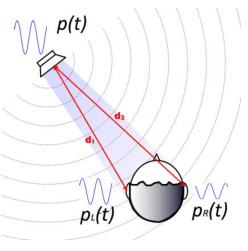
\includegraphics[width=6cm, height=6cm]{images/stereo_listening_mechanism.png}
  \caption{Απεικόνιση του μηχανισμού στερεοφωνικής ακρόασης}
  \label{fig:stereo_listening_mechanism}
\end{figure}

Οι ακροατές εντοπίζουν και διαφοροποιούν με ακρίβεια πηγές που δεν εμφανίζουν σχετικές διαφορές ηχοστάθμης ή/και φάσης στα δύο αυτιά (πχ μια πηγή που είναι ακριβώς μπροστά από το παρατηρητή και μια που είναι ακριβώς από πίσω του στην ίδια απόσταση), στην αντίληψη αξιοποιούνται επιπλέον φαινόμενα ανακλάσεων από τον άνω κορμό (ώμος, στήθος κλπ.) καθώς επίσης και την επίδραση του εξωτερικού πτερυγίου του αυτιού που συλλέγει και διαφοροποιεί τα ηχητικά κύματα που φτάνουν σε αυτό ανάλογα με τις διαφορετικές γωνίες πρόσπτωσης και στα δύο επίπεδα.

\subsection{Αμφιωτική ακρόαση}

Ο άνθρωπος ως ακουστικός δέκτης παρουσιάζει εξαιρετικές ικανότητες στην αναγνώριση και εντοπισμό ηχητικών πηγών στον τρισδιάστατο χώρο. Οι βασικές αρχές αντίληψης της θέσης των πηγών στον τρισδιάστατο χώρο που προαναφέρθηκαν και αφορούν τις σχετικές στάθμες, χρόνους άφιξης ενός σήματος στα 2 αυτιά, της σκίασης του κεφαλιού, της ως προς την γωνία φιλτραρίσματος του σήματος από το πτερύγιο του αυτιού και από τις ανακλάσεις στον άνω κορμό, μπορούν να γενικευθούν σε ένα πλαίσιο που συμπεριλαμβάνει όλους αυτούς τους καθοριστικούς μηχανισμούς και μπορούν να περιγράψουν την αμφιωτική ακρόαση.

Κατά τη γενική περίπτωση αμφιωτικής ακρόασης μιας ακουστικής πηγής, ο ήχος που φτάνει στα δύο αυτιά του ακροατή έχει σαν αποτέλεσμα την αντίληψη και τον προσδιορισμό της θέσης της πηγής σε κάποια γωνία τόσο στο οριζόντιο, όσο και στο κάθετο επίπεδο καθώς και την απόσταση που βρίσκεται αυτή (Σχήμα \ref{fig:binaural_perception_acoustic_source}). Η ικανότητα αυτή προκύπτει από την αντιληπτική διαδικασία που αξιοποιεί τη διαφοροποίηση των σημάτων που φτάνουν στα δύο αυτιά και είναι χαρακτηριστική τόσο για κάθε γωνία στο κάθετο, όσο και στο οριζόντιο επίπεδο. Η δυνατότητα εντοπισμού, εξαρτάται από την μορφολογία του πτερυγίου, του κεφαλιού και του άνω κορμού του εκάστοτε ακροατή. Η ευκρίνεια προσδιορισμού στο οριζόντιο επίπεδο είναι της τάξης των $5^o$ ενώ στο κάθετο επίπεδο είναι αρκετά χειρότερη.

Για την ανάλυση και την περιγραφή της αντιληπτικής διαδικασίας μέσω της δυϊκής θεωρίας, αξιοποιούνται η Αμφιωτική Διαφορά Στάθμης (ILD) και η Αμφιωτική Διαφορά Χρόνου (ITD) που αναλύονται στην ενότητα \ref{sec:binaural_cues}.

Οι δύο αυτές παράμετροι όμως δεν αρκούν για τον προσδιορισμό της θέσης μιας πηγής. Πρέπει να ληφθεί υπόψιν και η διαμόρφωση που εισάγει το εξωτερικό αυτί μέσω του σχήματος του πτερυγίου. Το προσπίπτον σήμα στο κάθε αυτί διαφοροποιείται και φασματικά, αναλόγως με τη γωνία πρόσπτωσης, λόγω της μορφολογίας του πτερυγίου του αυτιού που είναι χαρακτηριστική για κάθε άνθρωπο. Ο τρόπος που το εξωτερικό αυτί συνδυάζεται (μοντελοποιείται) μαζί με τις αμφιωτικές παραμέτρους που αναφέρθηκαν, αναλύονται στην ενότητα \ref{sec:HRTF}


\begin{figure}[h]
  \centering
  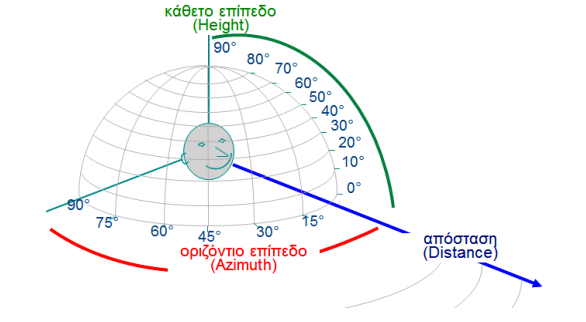
\includegraphics[width=\textwidth]{images/binaural_perception_acoustic_source.png}
  \caption{Αντίληψη και εντοπισμός θέσης πηγής μέσω αμφιωτικής ακρόασης}
  \label{fig:binaural_perception_acoustic_source}
\end{figure}